\documentclass[aspectratio=169,10pt]{beamer}

\usetheme{default}
\usecolortheme{default}
\setbeamertemplate{navigation symbols}{}
\setbeamertemplate{footline}[frame number]
\setbeamertemplate{itemize item}{\textbullet}
\setbeamertemplate{itemize subitem}{\textendash}

\definecolor{LaidlawNavy}{HTML}{1B2A41}
\definecolor{LaidlawTeal}{HTML}{3D6B6E}
\definecolor{LaidlawRust}{HTML}{A85A3A}
\definecolor{LaidlawGray}{HTML}{E8EAED}
\definecolor{LaidlawText}{HTML}{2C2C2C}
\definecolor{LaidlawSoft}{HTML}{F4F6F8}

\setbeamercolor{normal text}{fg=LaidlawText,bg=white}
\setbeamercolor{structure}{fg=LaidlawTeal}
\setbeamercolor{title}{fg=LaidlawNavy}
\setbeamercolor{frametitle}{fg=LaidlawNavy}
\setbeamerfont{frametitle}{series=\bfseries,size=\large}

\usepackage{booktabs}
\usepackage{graphicx}
\usepackage{microtype}
\usepackage{tikz}
\usepackage{array}
\usetikzlibrary{arrows.meta,positioning}
\setlength{\leftmargini}{1.15em}
\setlength{\itemsep}{0.28em}

\newcommand{\callout}[1]{%
  \begin{tikzpicture}
    \node[
      fill=LaidlawSoft,
      draw=LaidlawGray,
      rounded corners=2pt,
      inner xsep=8pt,
      inner ysep=5pt,
      text width=0.92\textwidth,
      align=left,
      font=\footnotesize
    ] {#1};
  \end{tikzpicture}%
}

\title{Week~2 Progress}
\author{Bob Shen}
\date{July 2026}
\institute{Laidlaw Scholars Programme $\cdot$ Bishai Lab}

\begin{document}

%======================================================================
\begin{frame}[plain]
  \vspace{1.8cm}
  {\color{LaidlawNavy}\LARGE\bfseries Week~2 Progress\par}

  \vspace{1.6em}
  {\normalsize Bob Shen\\[0.2em]
  Laidlaw Scholars Programme\\[0.2em]
  Bishai Lab\\[0.2em]
  July 2026\par}
\end{frame}

%----------------------------------------------------------------------
\begin{frame}{This is a team project}
  \begin{columns}[T]
    \begin{column}{0.48\textwidth}
      {\color{LaidlawTeal}\textbf{Hogan}}
      \begin{itemize}
        \item Weather and heat framing
        \item Goggins baseline challenge (Jan)
        \item Ages 65--69 and 70--74
        \item Climate $X$ file and hot-month definitions
      \end{itemize}
      \vspace{0.55em}
      {\color{LaidlawTeal}\textbf{Roro}}
      \begin{itemize}
        \item Hospital Authority stroke aggregates
        \item Outcome timing and transfer path
      \end{itemize}
    \end{column}
    \begin{column}{0.48\textwidth}
      {\color{LaidlawTeal}\textbf{Dr Bishai}}
      \begin{itemize}
        \item Original multi-method plan
        \item Teamwork: go far together
      \end{itemize}
      \vspace{0.55em}
      {\color{LaidlawTeal}\textbf{Also in the room this week}}
      \begin{itemize}
        \item Writing early (lit $+$ methods) matters
        \item Equity lens (Marmot): who bears risk
        \item Peer heat work: summit, district voice, LegCo
      \end{itemize}
    \end{column}
  \end{columns}

  \vspace{0.55em}
  \callout{This update credits the team's contributions.
  Judgments on weather and outcomes are still shared.}
\end{frame}

%----------------------------------------------------------------------
\begin{frame}{What the July meeting changed}
  \footnotesize
  \renewcommand{\arraystretch}{1.22}
  \begin{tabular}{@{}p{0.30\textwidth}p{0.32\textwidth}p{0.30\textwidth}@{}}
    \toprule
    \textbf{Earlier plan} & \textbf{Meeting} & \textbf{Working now} \\
    \midrule
    AMI $+$ stroke principal-dx & No admission reasons in general HA file & Stroke aggregates; AMI out of scope from that file \\[0.4em]
    One primary heat model & Explore many methods & Labelled multi-spec panel \\[0.4em]
    Heat metrics & Align with Ren/Wang-style spells & Spells, 2D3N, hot-month options with Hogan \\
    \bottomrule
  \end{tabular}

  \vspace{0.55em}
  \callout{\textbf{Roro's outcome path (working understanding):}
  first GOPC mention of stroke is a \emph{marker}.
  The actual stroke and hospitalisation generally come earlier.
  We ignore later mentions and work back to the true event month.}
\end{frame}

%----------------------------------------------------------------------
\begin{frame}{The question we are preparing}
  \vspace{0.2em}
  \begin{center}
  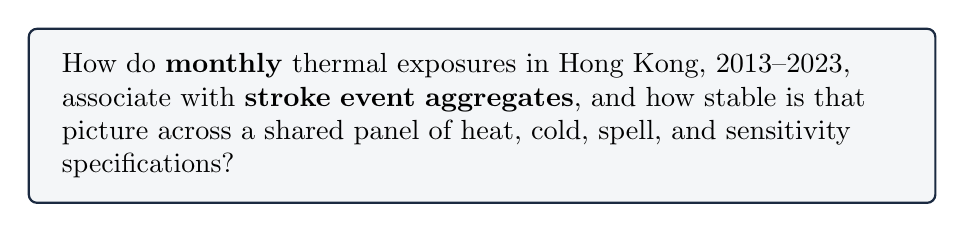
\begin{tikzpicture}
    \node[
      fill=LaidlawSoft,
      draw=LaidlawNavy,
      line width=0.8pt,
      rounded corners=3pt,
      inner xsep=12pt,
      inner ysep=9pt,
      text width=0.88\textwidth,
      align=left,
      font=\normalsize
    ] {%
      How do \textbf{monthly} thermal exposures in Hong Kong, 2013--2023,
      associate with \textbf{stroke event aggregates},
      and how stable is that picture across a shared panel of
      heat, cold, spell, and sensitivity specifications?
    };
  \end{tikzpicture}
  \end{center}

  \vspace{0.55em}
  \footnotesize
  Complementary to daily heatwave--mortality work in the lab --- not a duplicate.
  Not a daily DLNM; not AMI from a file without admission reasons.
\end{frame}

%----------------------------------------------------------------------
\begin{frame}{From January: Hogan's intellectual lead}
  \footnotesize
  \begin{itemize}
    \item Pulled Goggins MI (2013) and stroke (2012) as the Hong Kong baseline
    \item Warned that cold associations are already well documented --- novelty must be careful
    \item Suggested comparing a later period (2013--2023) as an evolutionary question
    \item Highlighted ages \textbf{65--69} and \textbf{70--74} as actionable older bands
    \item Offered to prepare the monthly climate $X$ file under Dr Bishai's plan
    \item Later: define heatwaves, count them by month, flag upper-tail ``hot'' months
      (Atmos.\ Res.\ heatwave framing; DOI 10.1016/j.atmosres.2024.107845)
  \end{itemize}

  \vspace{0.4em}
  \callout{Those contributions still structure the weather side.
  Definitions should be finished \textbf{with} Hogan, not around him.}
\end{frame}

%----------------------------------------------------------------------
\begin{frame}{Climate: shared ground truth (descriptive)}
  \begin{center}
    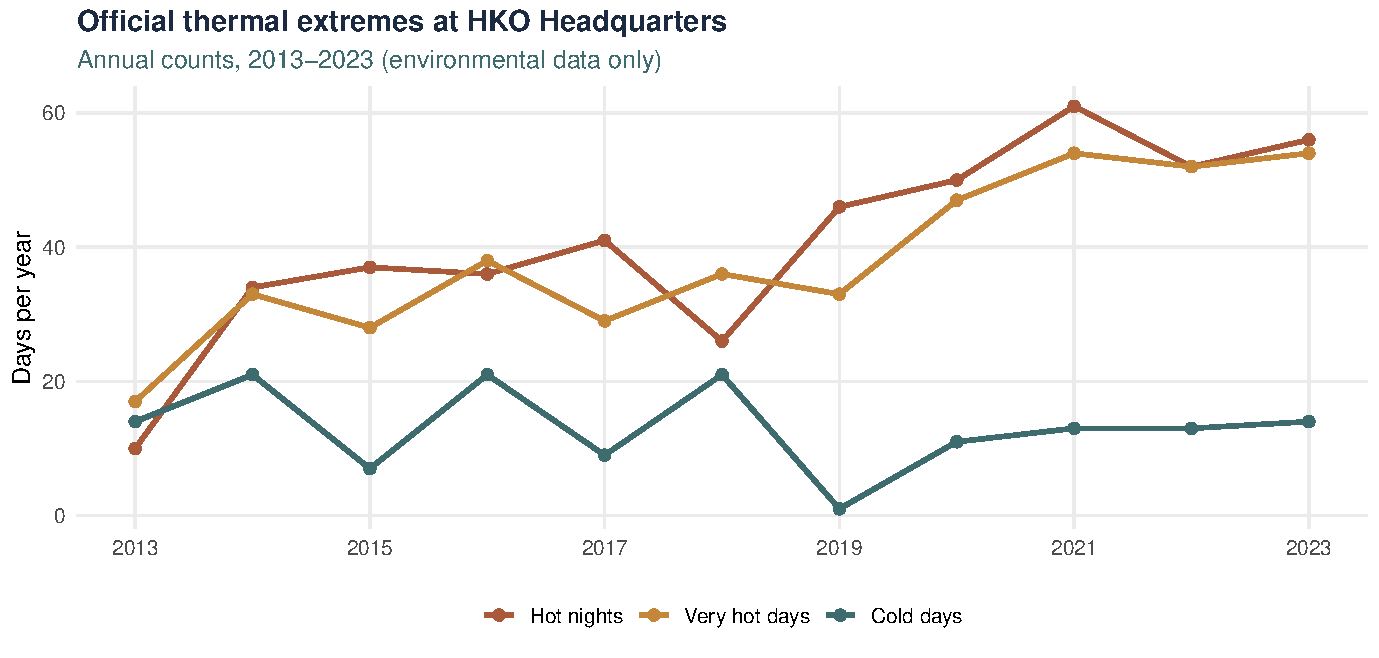
\includegraphics[width=0.94\textwidth]{../../figures/week2_progress/fig_annual_extremes.pdf}
  \end{center}
  \vspace{-0.15em}
  \begin{center}
  \scriptsize
  Hot nights and very hot days rose after 2018; cold days persist.
  Peak hot-night year in-window: \textbf{2021 (61)}.
  Environmental descriptives only --- no stroke findings.
  \end{center}
\end{frame}

%----------------------------------------------------------------------
\begin{frame}{Pollution layer (EPD EPIC)}
  \begin{center}
    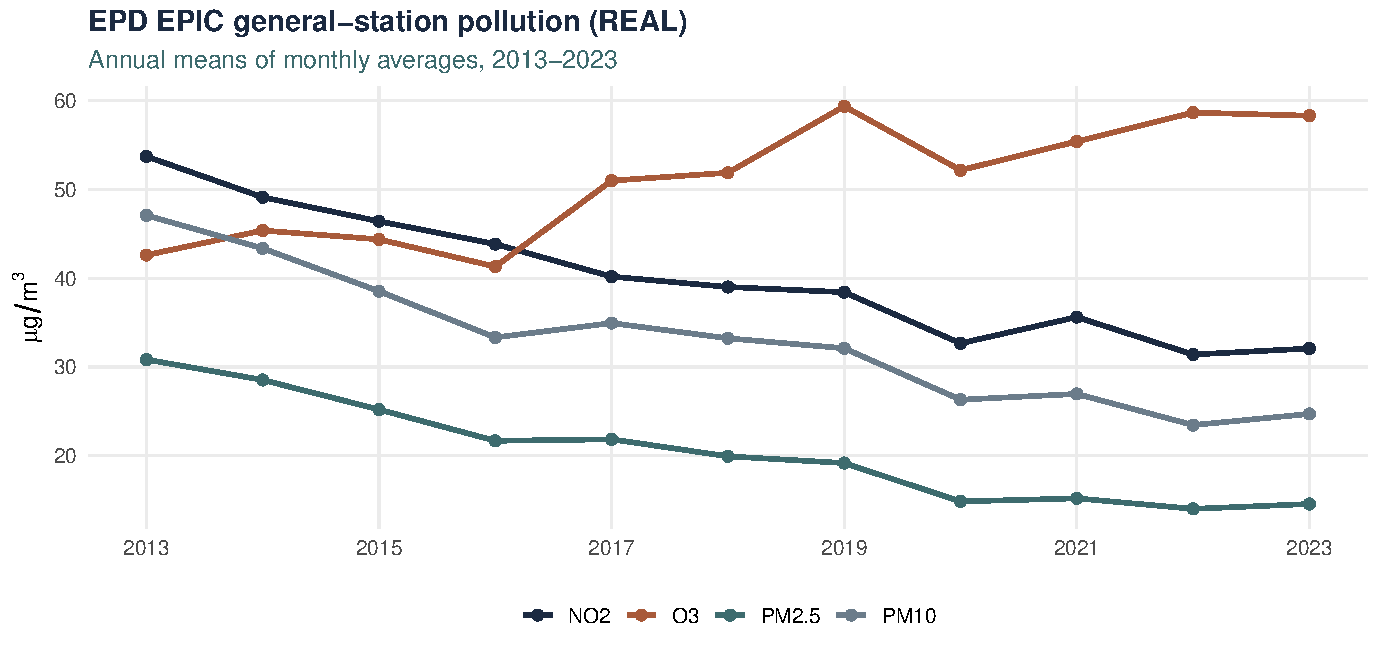
\includegraphics[width=0.90\textwidth]{../../figures/week2_progress/fig_pollution_annual.pdf}
  \end{center}
  \vspace{-0.15em}
  \footnotesize
  Official monthly general-station means: NO$_2$, O$_3$, PM$_{2.5}$, PM$_{10}$.
  NO$_2$/PM declined; O$_3$ rose --- echoing the January discussion of a changing pollutant mix.
  Stage pollutants carefully; enter O$_3$ last.
\end{frame}

%----------------------------------------------------------------------
\begin{frame}{Why heatwave definitions stay plural}
  \begin{center}
    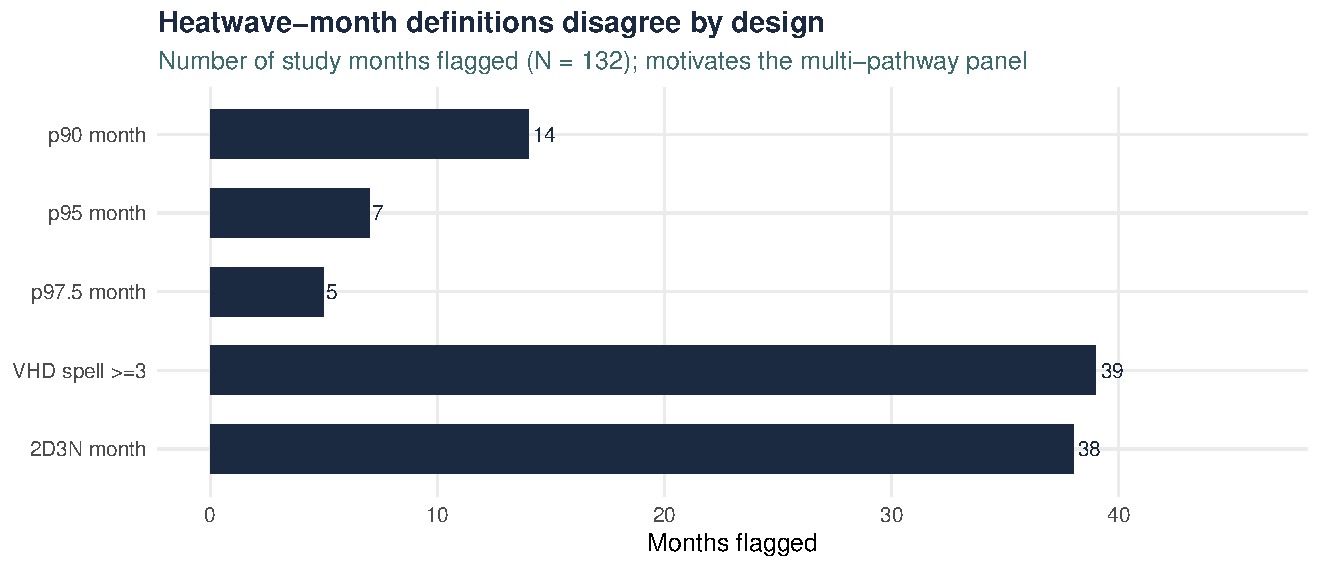
\includegraphics[width=0.86\textwidth]{../../figures/week2_progress/fig_hw_month_defs.pdf}
  \end{center}
  \vspace{0.1em}
  \footnotesize
  Guo/Gasparrini, Wang/Ren, and the lab's multi-definition mortality work all argue against one universal rule.
  \textbf{Hogan's hot-month idea} (heatwave counts $\to$ upper-tail months) belongs here as a named option.
\end{frame}

%----------------------------------------------------------------------
\begin{frame}{A labelled panel --- not seventeen discoveries}
  \footnotesize
  \renewcommand{\arraystretch}{1.1}
  \begin{tabular}{@{}p{0.34\textwidth}p{0.58\textwidth}@{}}
    \toprule
    \textbf{Family} & \textbf{Examples (lit-anchored)} \\
    \midrule
    Continuous T / lag & Tmean; Tmax/Tmin; lag-1 \\
    Official extremes & Hot nights, very hot days, cold days (Hogan / HKO) \\
    Spells \& 2D3N & Ren/Wang-style burden metrics \\
    Hot-month defs & Percentile months $+$ Hogan count$\to$tail idea \\
    Cold \& flu & Cold-primary; influenza co-exposure \\
    Structure & Age bands Hogan flagged; sex if grain allows \\
    Sensitivities & Pollution staging; humidity; COVID window \\
    \bottomrule
  \end{tabular}

  \vspace{0.45em}
  \callout{Headline proposal for Gate~3 \emph{with the team}:
  continuous Tmax/Tmin $+$ official extreme-day counts.
  Full pathway$\times$literature map is in the Laidlaw write-up.}
\end{frame}

%----------------------------------------------------------------------
\begin{frame}{What each person still unlocks}
  \begin{center}
    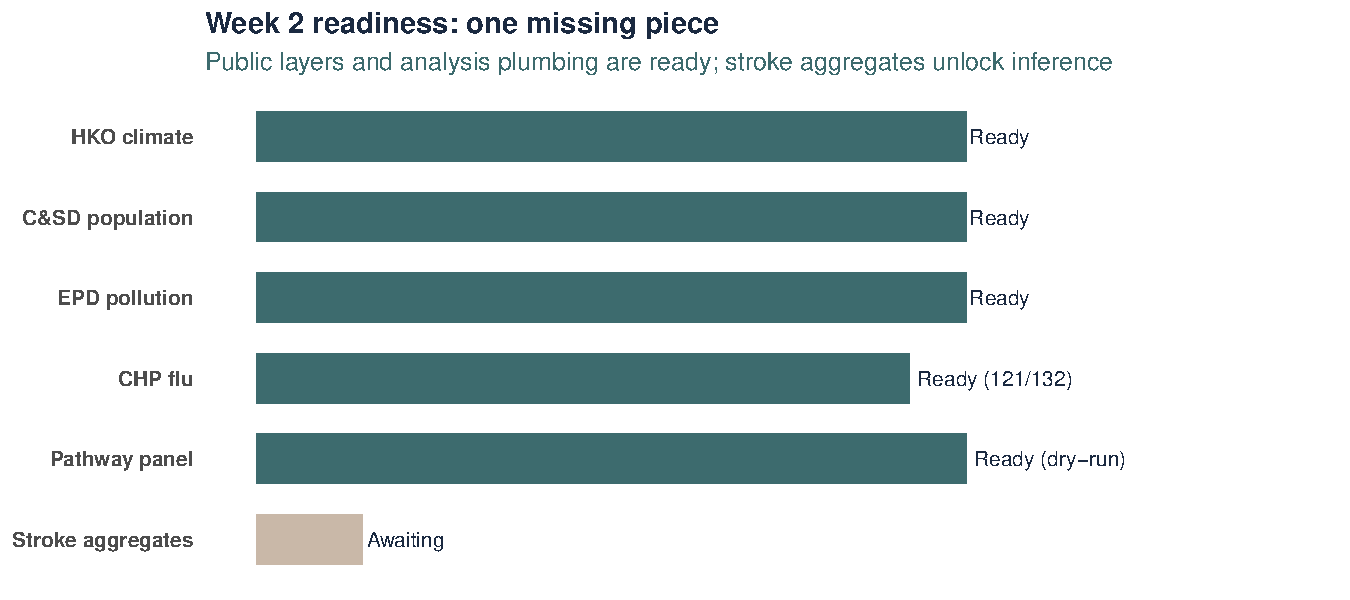
\includegraphics[width=0.88\textwidth]{../../figures/week2_progress/fig_readiness.pdf}
  \end{center}
  \vspace{0.1em}
  \footnotesize
  {\color{LaidlawTeal}\textbf{Hogan:}} final weather / heatwave / hot-month operationalisation.\\
  {\color{LaidlawTeal}\textbf{Roro:}} stroke aggregates --- first GOPC mention $\to$ true event month; dictionary; transfer.\\
  Public pollution and population layers can support the merge once outcomes arrive.
\end{frame}

%----------------------------------------------------------------------
\begin{frame}{Honesty line}
  \begin{columns}[T]
    \begin{column}{0.50\textwidth}
      {\color{LaidlawTeal}\textbf{Ready to discuss}}
      \begin{itemize}
        \item Environmental descriptives
        \item Outcome construction logic with Roro
        \item Weather definitions with Hogan
        \item Lit $+$ methods writing for Laidlaw
      \end{itemize}
    \end{column}
    \begin{column}{0.48\textwidth}
      {\color{LaidlawRust}\textbf{Not ready to claim}}
      \begin{itemize}
        \item Stroke coefficients
        \item ``Heat replaced cold''
        \item AMI from this HA file
        \item Synthetic dry-runs as findings
      \end{itemize}
    \end{column}
  \end{columns}
\end{frame}

%----------------------------------------------------------------------
\begin{frame}{Literature anchors (selected)}
  \footnotesize
  \begin{itemize}
    \item \textbf{Goggins 2012/2013} --- cold-dominant HK stroke/AMI baselines (Hogan's challenge)
    \item \textbf{Guo 2024} --- hot-night intensity vs official binary flags
    \item \textbf{Wang/Ren 2019} --- VHD/HN spells and 2D3N
    \item \textbf{Guo/Gasparrini 2017} --- multi-definition heatwaves
    \item \textbf{Yang/Chong 2025} --- cold $+$ influenza and stroke
    \item \textbf{Guo 2025} --- pollution can amplify temperature--hospitalisation risks
  \end{itemize}
\end{frame}

%----------------------------------------------------------------------
\begin{frame}{Laidlaw Stage~3 is on the horizon}
  \footnotesize
  \begin{itemize}
    \item Research essay (2000--3000 words) --- lit $+$ methods drafts are started
    \item A0 \textbf{portrait} poster (841$\times$1189\,mm) --- research focus; results pending outcomes
    \item HKU report form $+$ supervisor endorsement
    \item Showcase: HKU Laidlaw Society (early Nov 2026) and Annual Conference
  \end{itemize}

  \vspace{0.55em}
  \callout{Writing early --- as other presenters modelled --- is how we stay honest
  about what is ready and what still needs the team.}
\end{frame}

%----------------------------------------------------------------------
\begin{frame}[plain]
  \vspace{1.1cm}
  {\color{LaidlawNavy}\LARGE\bfseries Thank you\par}
  \vspace{0.55em}
  {\large\color{LaidlawTeal}
  Next small asks --- whenever you have a moment :)\par}

  \vspace{0.85em}
  \footnotesize
  \begin{itemize}
    \item \textbf{Hogan:} shall we lock the heatwave / hot-month definitions together
      (including your count$\to$upper-tail idea)?
    \item \textbf{Roro:} when you can, a short note on the first-GOPC$\to$true-stroke timing
      and the aggregate file path would unlock the merge.
  \end{itemize}

  \vspace{1.0em}
  {\small
  If you want to go fast, go alone; if you want to go far, go together.\\[0.25em]
  Grateful for both of you --- and for Dr Bishai's nudge to listen better.
  \par}
\end{frame}

\end{document}
